\section{Implementation and Measured Results}
\label{sec:impl}
This section reports the system as built and what it measured, as of 18 October 2026. Phases~0--6 of the
roadmap are implemented on the CPU reference machine, and a Phase~7 on CPU inference performance was added
(Section~\ref{sec:impl:perf}). GPU training and GPU scale-out were deferred. Every number below is generated by
\texttt{scripts/gen\_publication.py} from stored runs and evidence files. The machine was shared with other
workloads (load average 6--18), so absolute speeds are lower bounds and small effects are within noise. Sample
sizes are far below the release gates of Section~\ref{sec:eval}, so the results are indicative.

\subsection{The system as built}
The Rust workspace has eight crates: the gateway (axum), the orchestrator (\texttt{nafs-core}), verifiers with
a sandbox, memory (SQLite, BM25 retrieval), evaluation and statistics, load testing, the shared types, and an
embedded web interface. The gateway serves 50 documented endpoints (OpenAPI~1.5) and an OpenAI-compatible chat
API. System~1 is Qwen3-1.7B and System~2 Qwen3-4B-Thinking-2507, both in Q4\_K\_M on llama-server; a vLLM-CPU
profile runs the same API in a Linux VM or container.

The web interface (Fig.~\ref{fig:ui-chat}) has seven pages:
\begin{itemize}
\item \textbf{Chat:} streaming answers with the automaton strip (A~$\to$~L~$\to$~M~$\to$~T/X), assurance badges,
a one-line reason from the gate, an inspector with the decision record and a per-stage latency waterfall, and
``Both'' trials in which a person compares the System~1 and System~2 answers;
\item \textbf{Lab:} experiment presets, paired statistics, the roadmap gates and a pooled policy map;
\item \textbf{Muhasaba:} gate mode and calibration, verifier quality, the capability ledger, drift and alerts;
\item \textbf{Tazkiya:} distillation readiness, the review queue and the model registry;
\item \textbf{Rooms}, \textbf{Performance} and \textbf{System}.
\end{itemize}

\begin{figure*}[t]
\centering
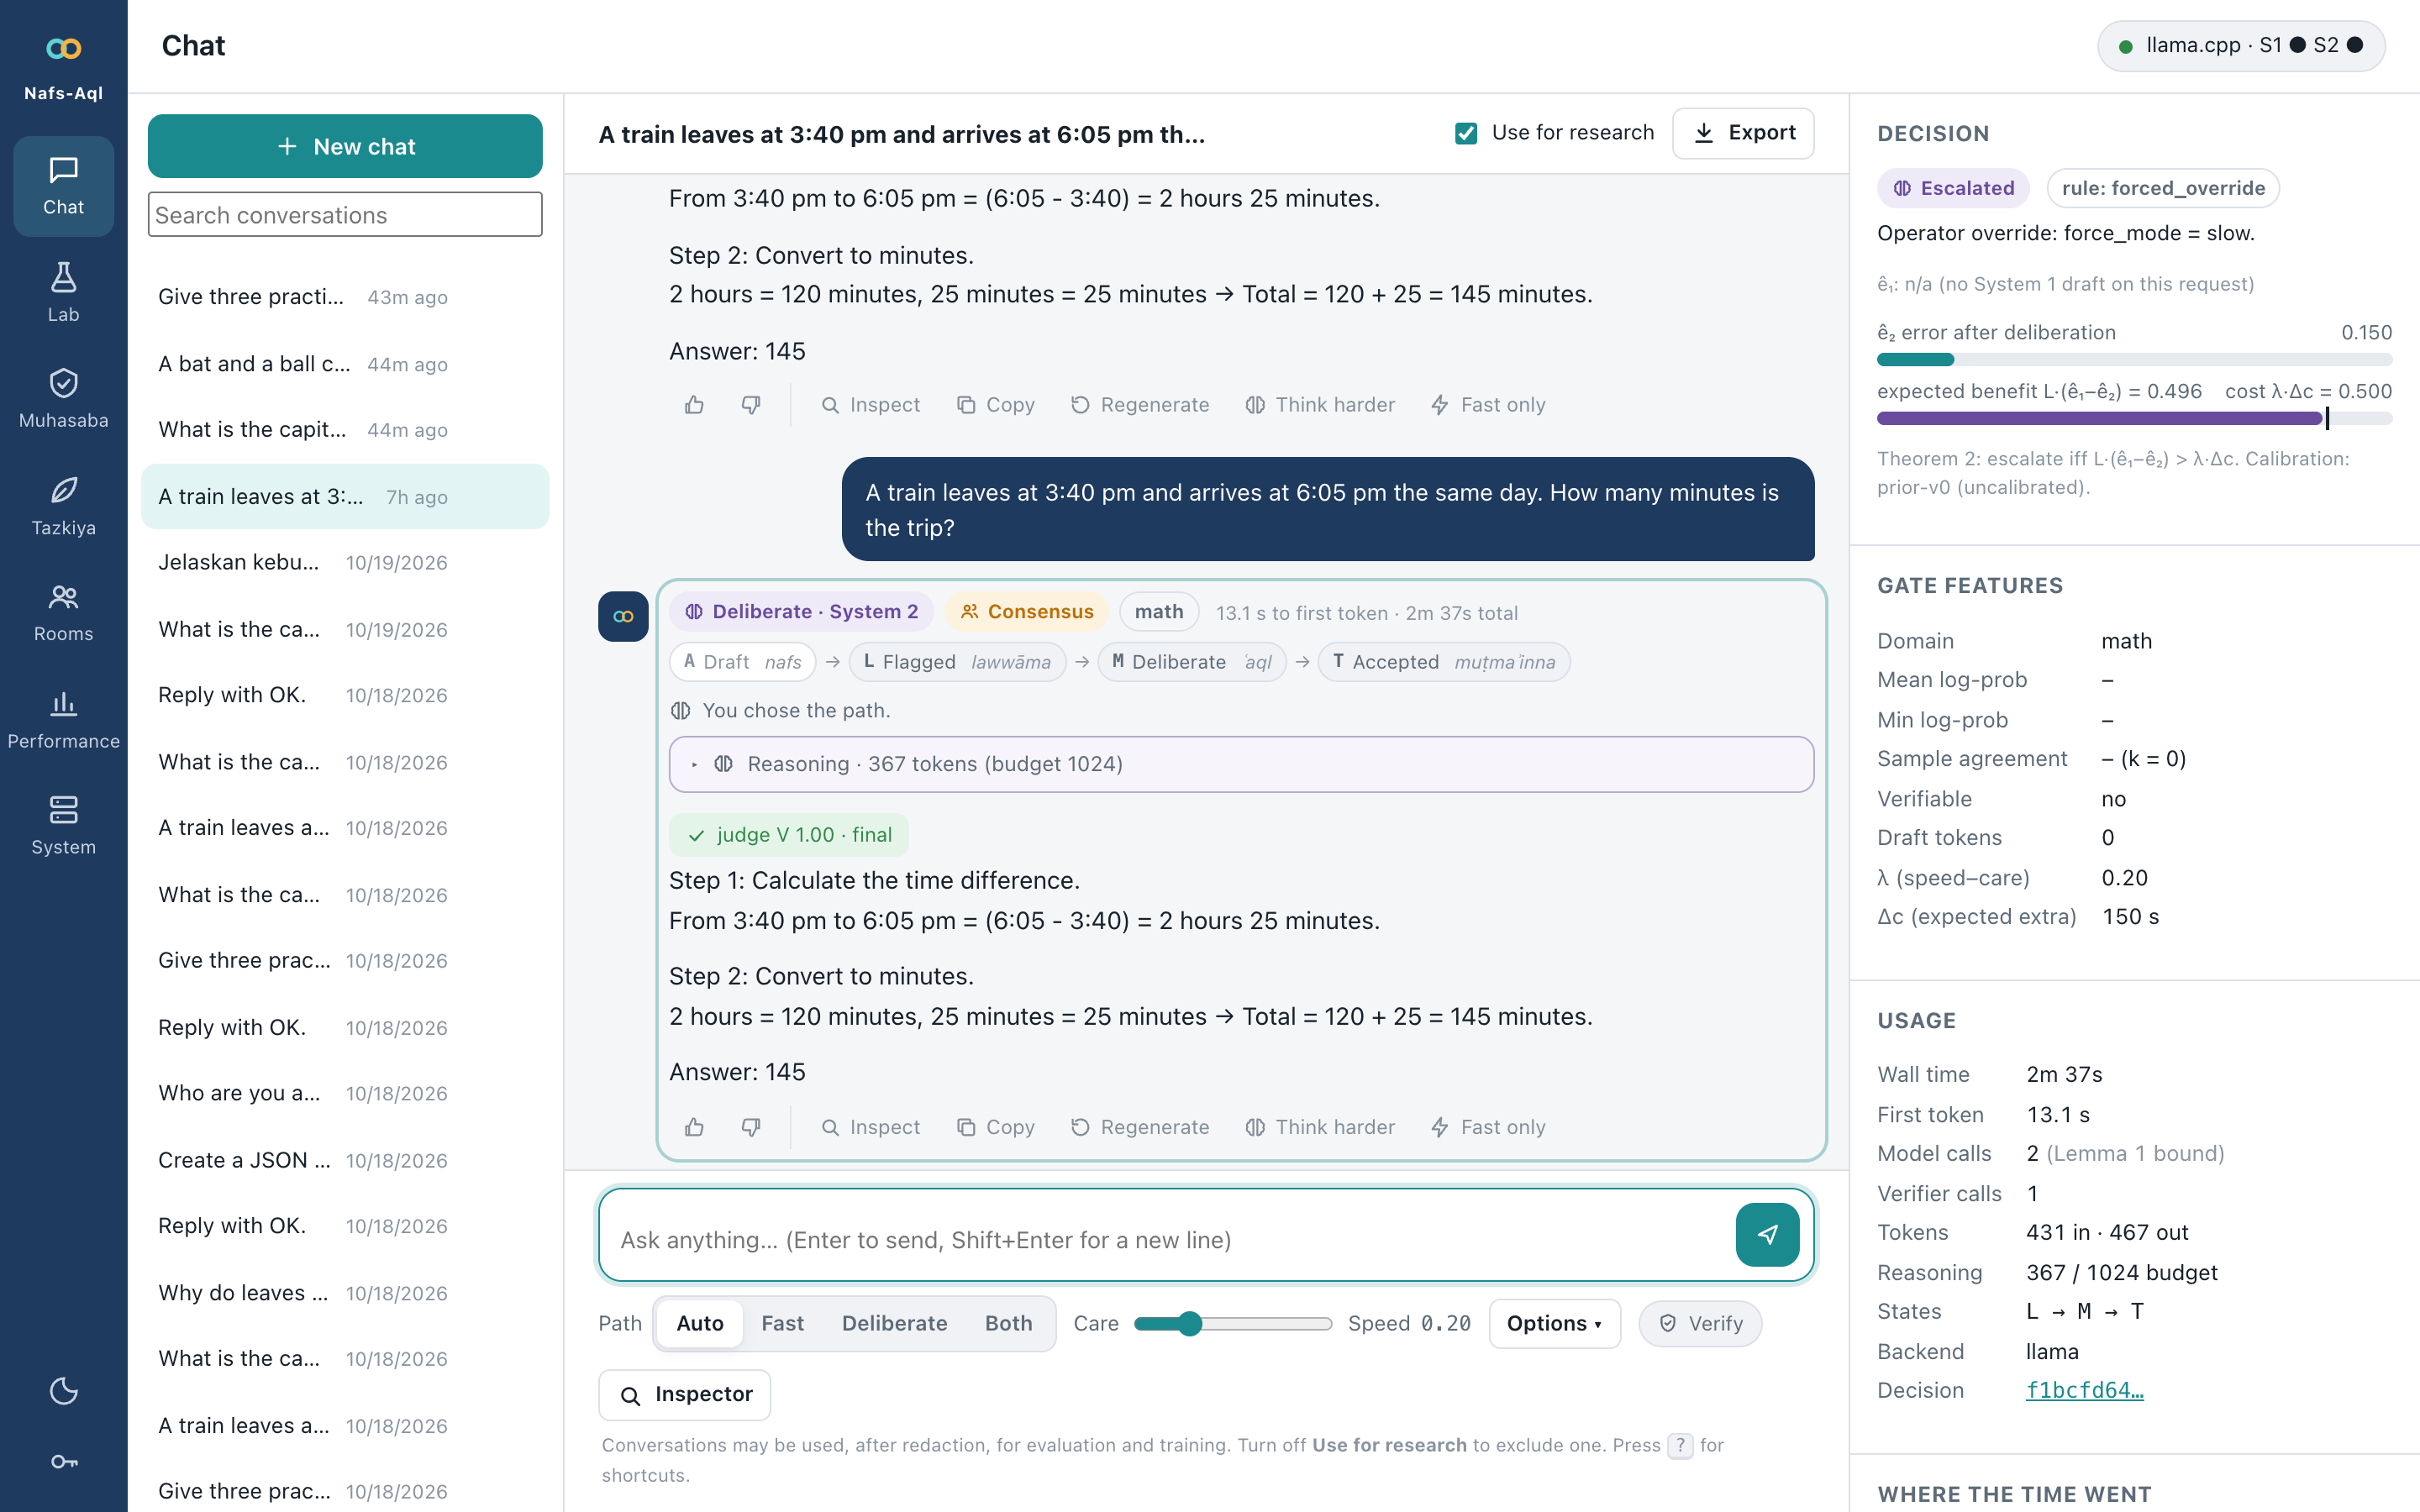
\includegraphics[width=0.9\textwidth]{../shared/screenshots/chat.png}
\caption{Chat page (measured system). A code answer passed the exact verifier on the draft, so the gate kept it
(Theorem~1); the inspector shows the decision, the gate features and the usage.}
\label{fig:ui-chat}
\end{figure*}

\subsection{The laboratory}
The Lab treats each way of combining the two systems as a \emph{policy} and runs them on identical tasks:
\begin{itemize}
\item fast only and deliberate only;
\item the gate with the verifier visible, and the gate routing on its own estimate (``blind'');
\item a draft-conditioned ablation;
\item thinking-budget and $\lambda$ sweeps.
\end{itemize}
Paired differences carry bootstrap intervals, exact McNemar tests and Bonferroni correction. The \emph{policy
map} (Fig.~\ref{fig:ui-lab}) pools every stored run and, for each domain and each price of latency $\lambda$,
names the policy with the lowest expected loss $L(1-\mathrm{acc})+\lambda c$. Over the \PolicyMapRuns{} stored
runs the best policy is, per domain: \PolicyMapSummary. Below a price of about 0.1 per minute of waiting, deliberation
pays for its time on code and mathematics. Above it, the fast path wins, because the verifier already catches most
of its errors.

\begin{figure*}[t]
\centering
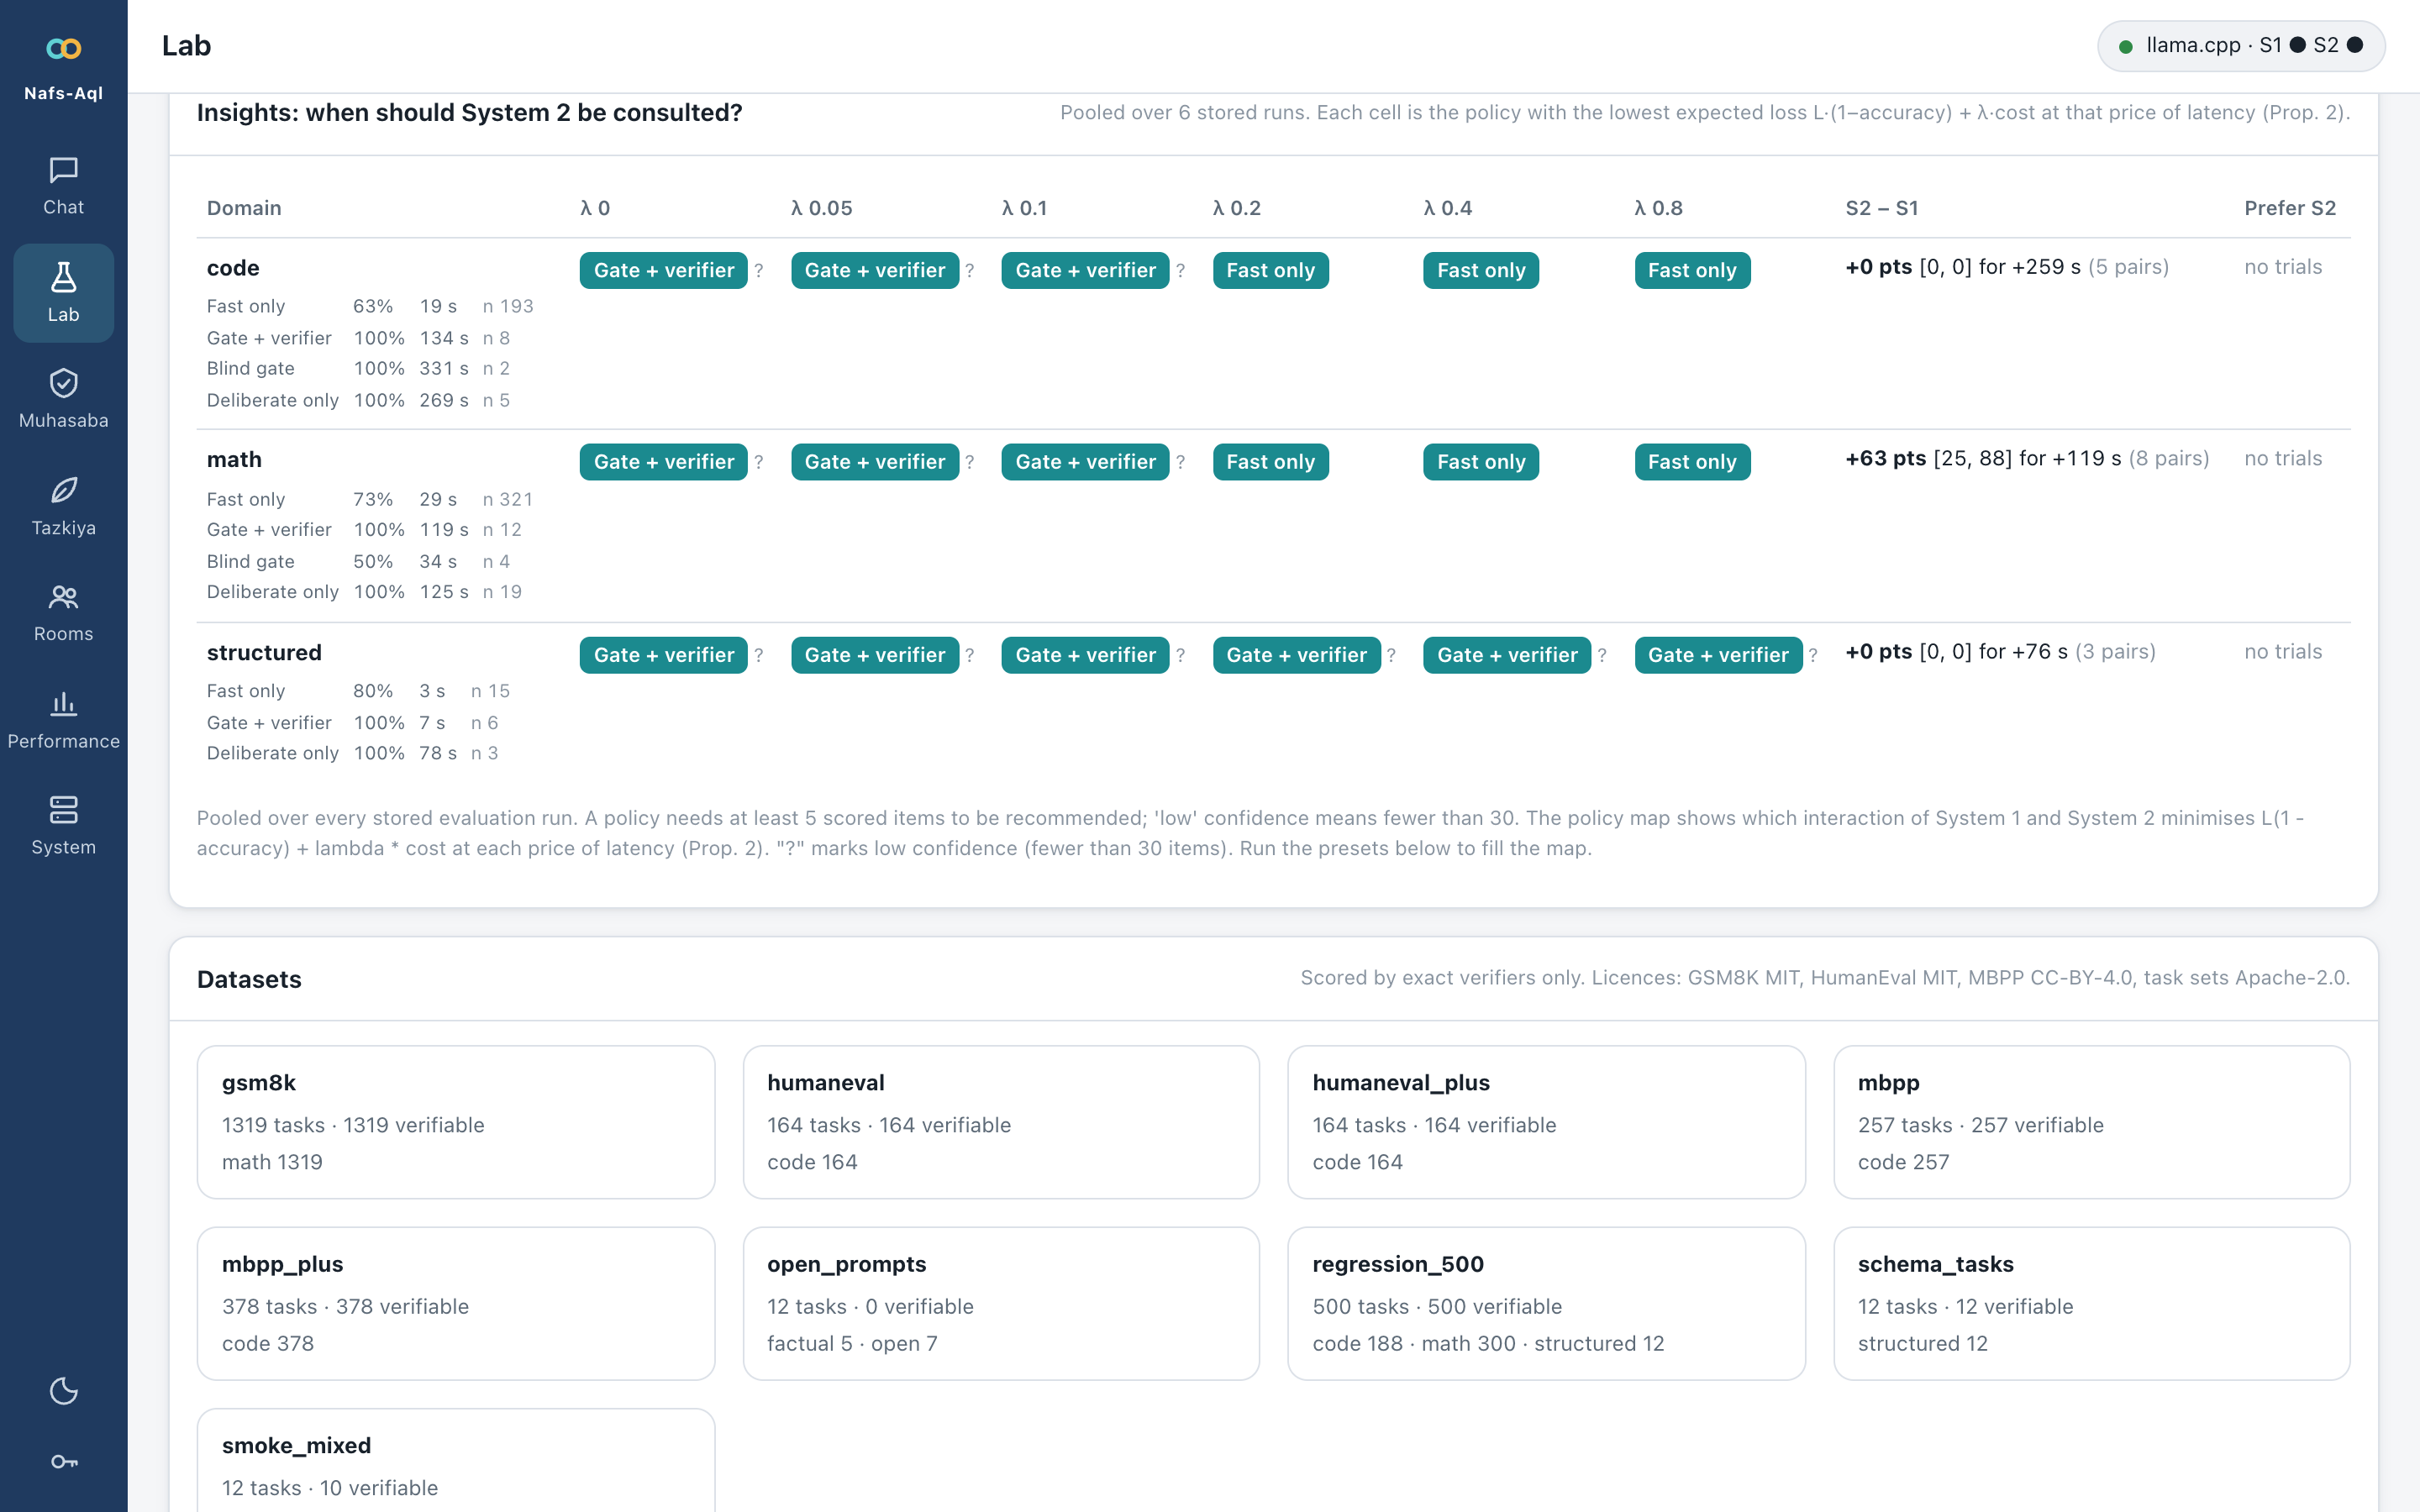
\includegraphics[width=0.48\textwidth]{../shared/screenshots/lab_insights.png}\hfill
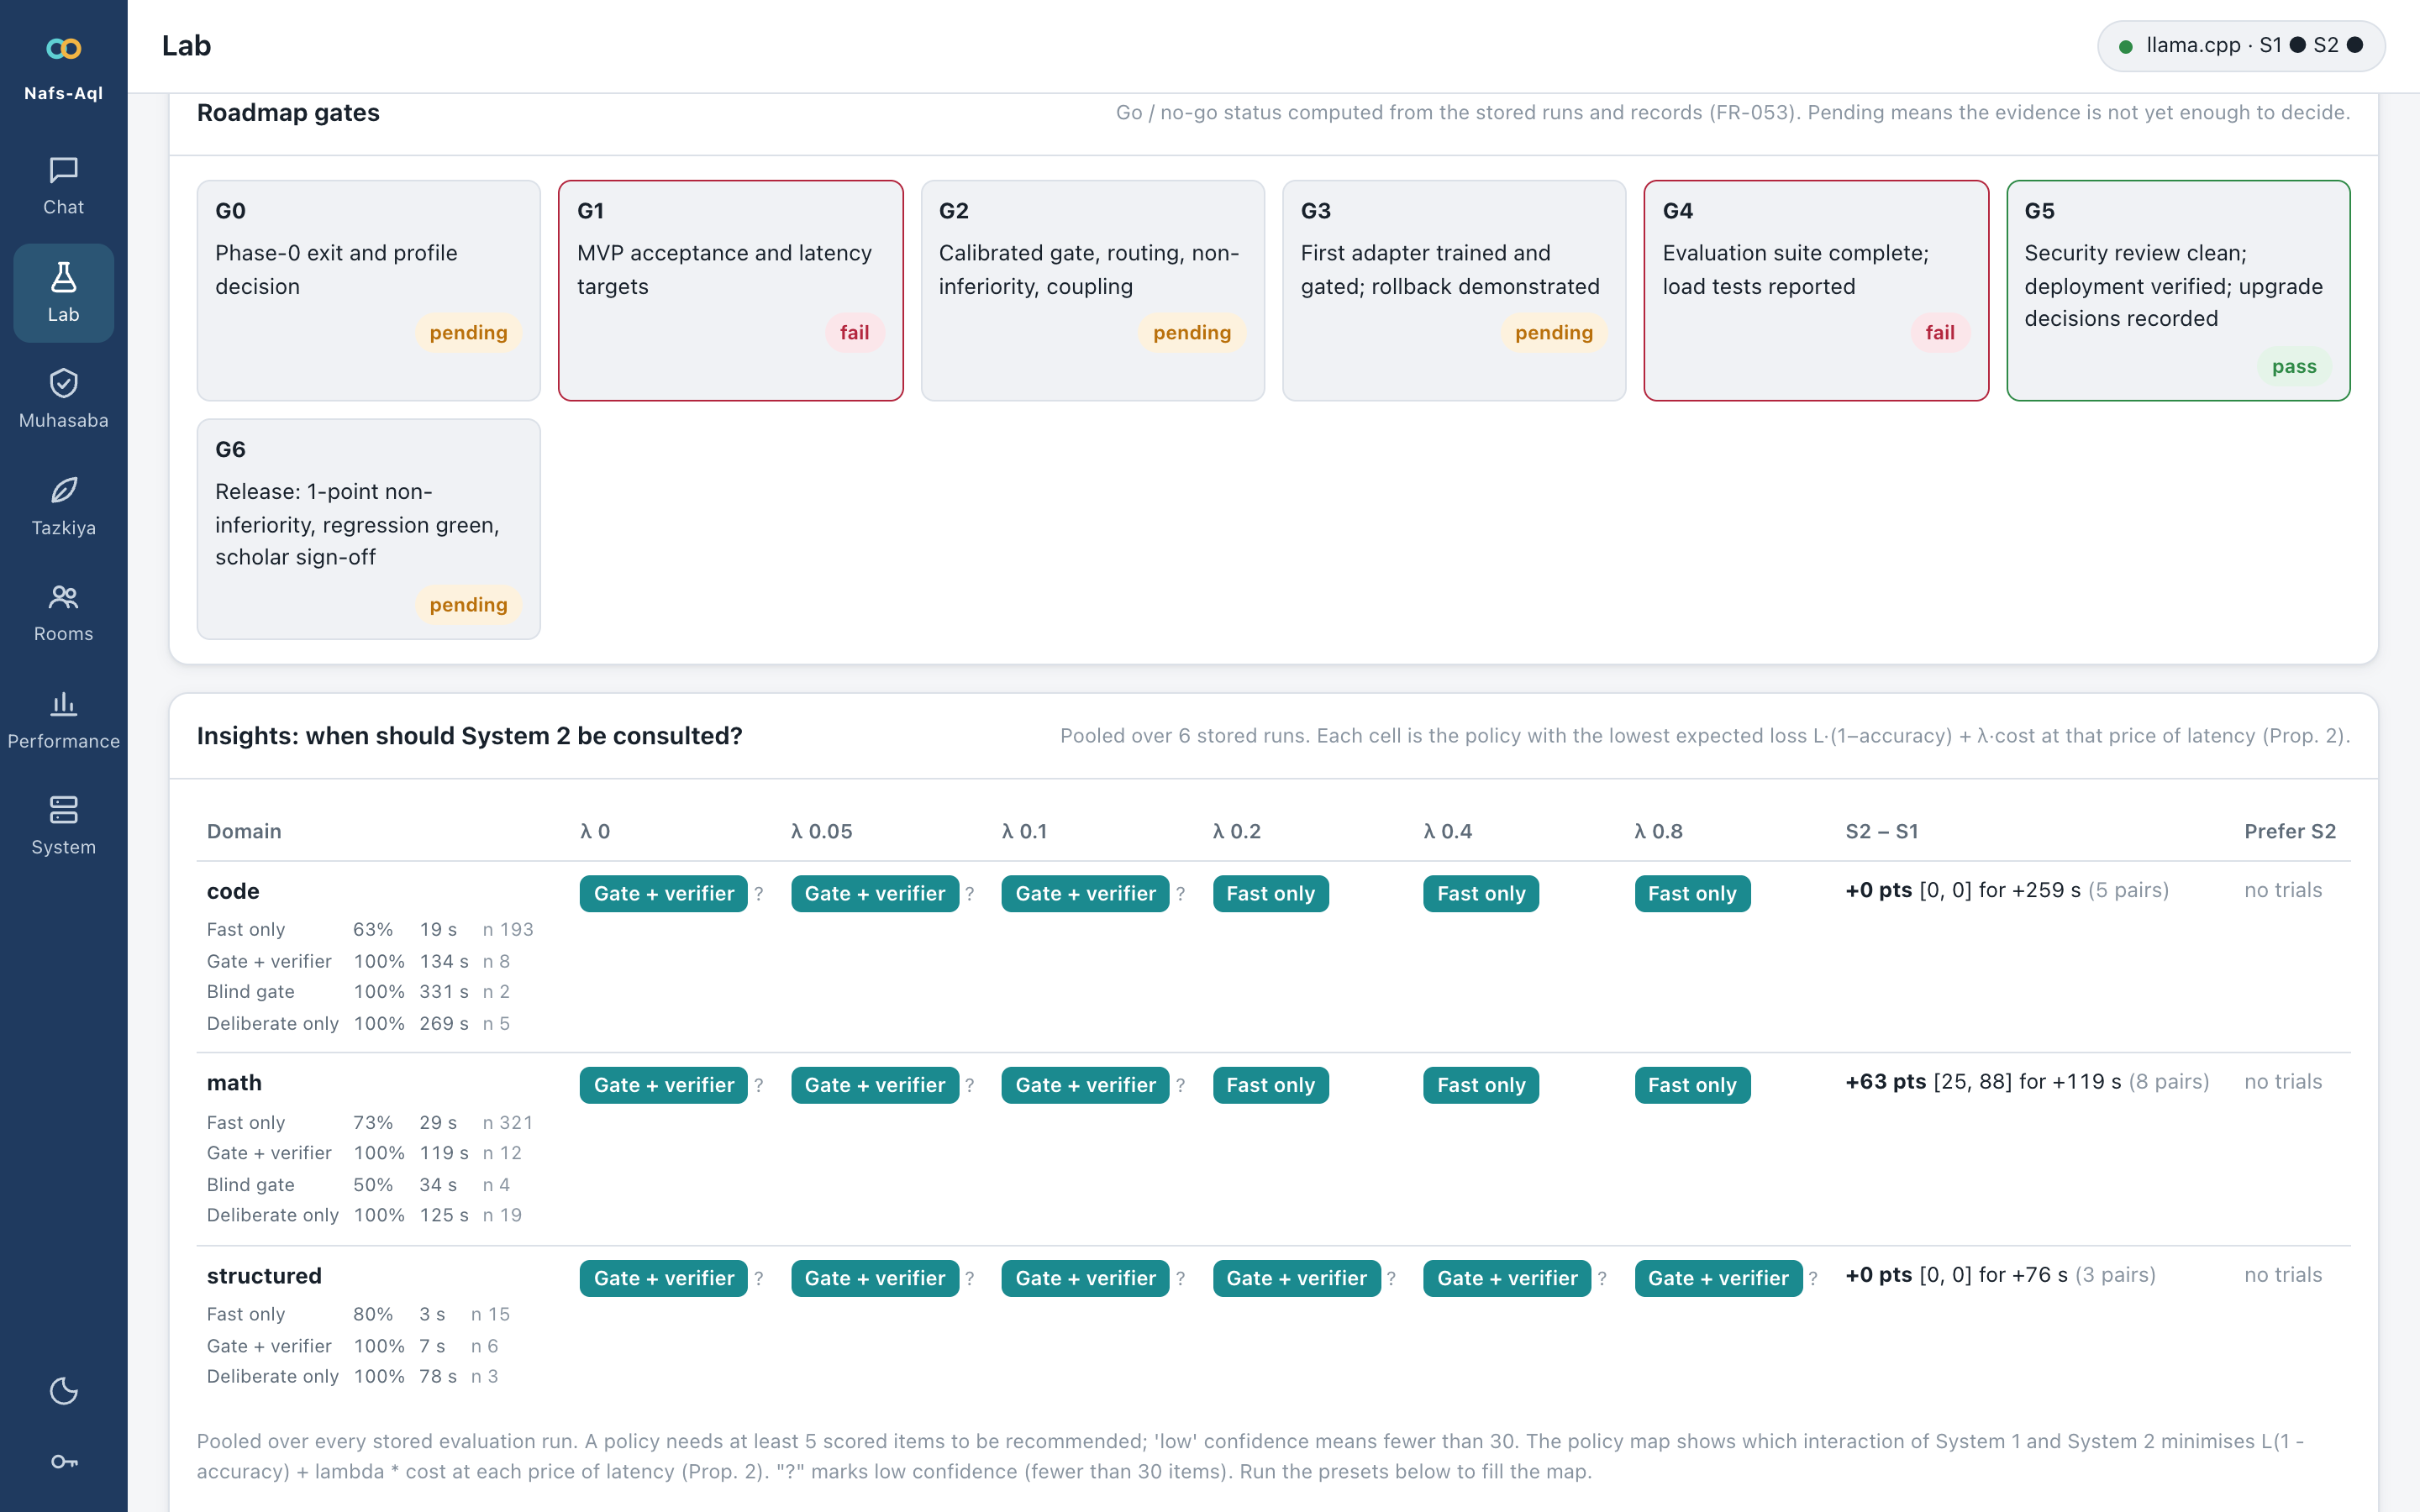
\includegraphics[width=0.48\textwidth]{../shared/screenshots/lab_gates.png}
\caption{Lab page: the pooled policy map, answering ``when should System~2 be consulted?'' per domain and price
of latency (left); roadmap gates G0--G6 evaluated from stored evidence (right).}
\label{fig:ui-lab}
\end{figure*}

\subsection{Policies, verifiers and model choice}
Table~\ref{tab:policies} shows one scaled run of five policies (run \PhaseTwoRun). With the verifier visible,
the gate matched deliberate-only accuracy at \GatedCostRatio{} of its cost. With the verifier hidden, the
uncalibrated gate routed correctly on only \BlindRouting{} of items, because cheap samples agreed with wrong
drafts: agreement is a flag, not evidence (Theorem~\ref{thm:plurality}).

Table~\ref{tab:verifiers} gives the verifiers' measured true- and false-accept rates (runs \RatesRuns).
Mathematics meets the $\varphi\le0.01$ target. The code $\varphi$ is an upper bound inflated by behaviourally
equivalent mutants.

\begin{table}[t]
\centering\caption{Policies on a mixed task set (run \PhaseTwoRun)}\label{tab:policies}
\resizebox{\columnwidth}{!}{\PhaseTwoTable}
\end{table}

\begin{table}[t]
\centering\caption{Verifier quality: $r$ from correct answers, $\varphi$ from seeded mutants}\label{tab:verifiers}
\resizebox{\columnwidth}{!}{\VerifierTable}
\end{table}

The Profile~C decision (MR-005) compared Qwen3.5-2B with Qwen3-1.7B as System~1 on 30 tasks, in alternating
order and with the production prompt (Table~\ref{tab:profilec}). Qwen3.5-2B was more accurate
(\ProfileCDelta), but about 3.7 times slower per task under load. The adoption rule requires latency within
1.3 times, so Profile~A stays the default. The accuracy gain is recorded for a faster host.

\begin{table}[t]
\centering\caption{Profile~C decision (System~1 candidates, 30 tasks)}\label{tab:profilec}
\resizebox{\columnwidth}{!}{\ProfileCTable}
\end{table}

\subsection{CPU inference performance (Phase~7)}
\label{sec:impl:perf}
\textbf{Where the time goes.} Every reply now records its stages:
\begin{itemize}
\item retrieval, the System~1 draft, the cheap samples, verification, System~2 deliberation and the judge;
\item for each model stage, the gateway queue wait and llama-server's own prefill time, decode time and
KV-cache reuse.
\end{itemize}
Over \StageReplies{} replies with stage timings, the fast path spends essentially all of its time in the System~1
draft, and the deliberate path in System~2 deliberation (Table~\ref{tab:stages}, Fig.~\ref{fig:ui-perf}); verification and gating are negligible. The prompt cache already serves most prompt tokens
(Table~\ref{tab:engine}), so prefill is small. \emph{Decode speed is the bottleneck}, and it falls several-fold
when other workloads share the four cores: 2.6--4.3 tokens/s in service, against 22.9 in an idle llama-bench run.

\begin{table}[t]
\centering\caption{Latency by stage (share of wall time)}\label{tab:stages}
\resizebox{\columnwidth}{!}{\StageTable}
\end{table}
\begin{table}[t]
\centering\caption{Engine speed per model stage (llama-server timings)}\label{tab:engine}
\resizebox{\columnwidth}{!}{\EngineTable}
\end{table}

\begin{figure*}[t]
\centering
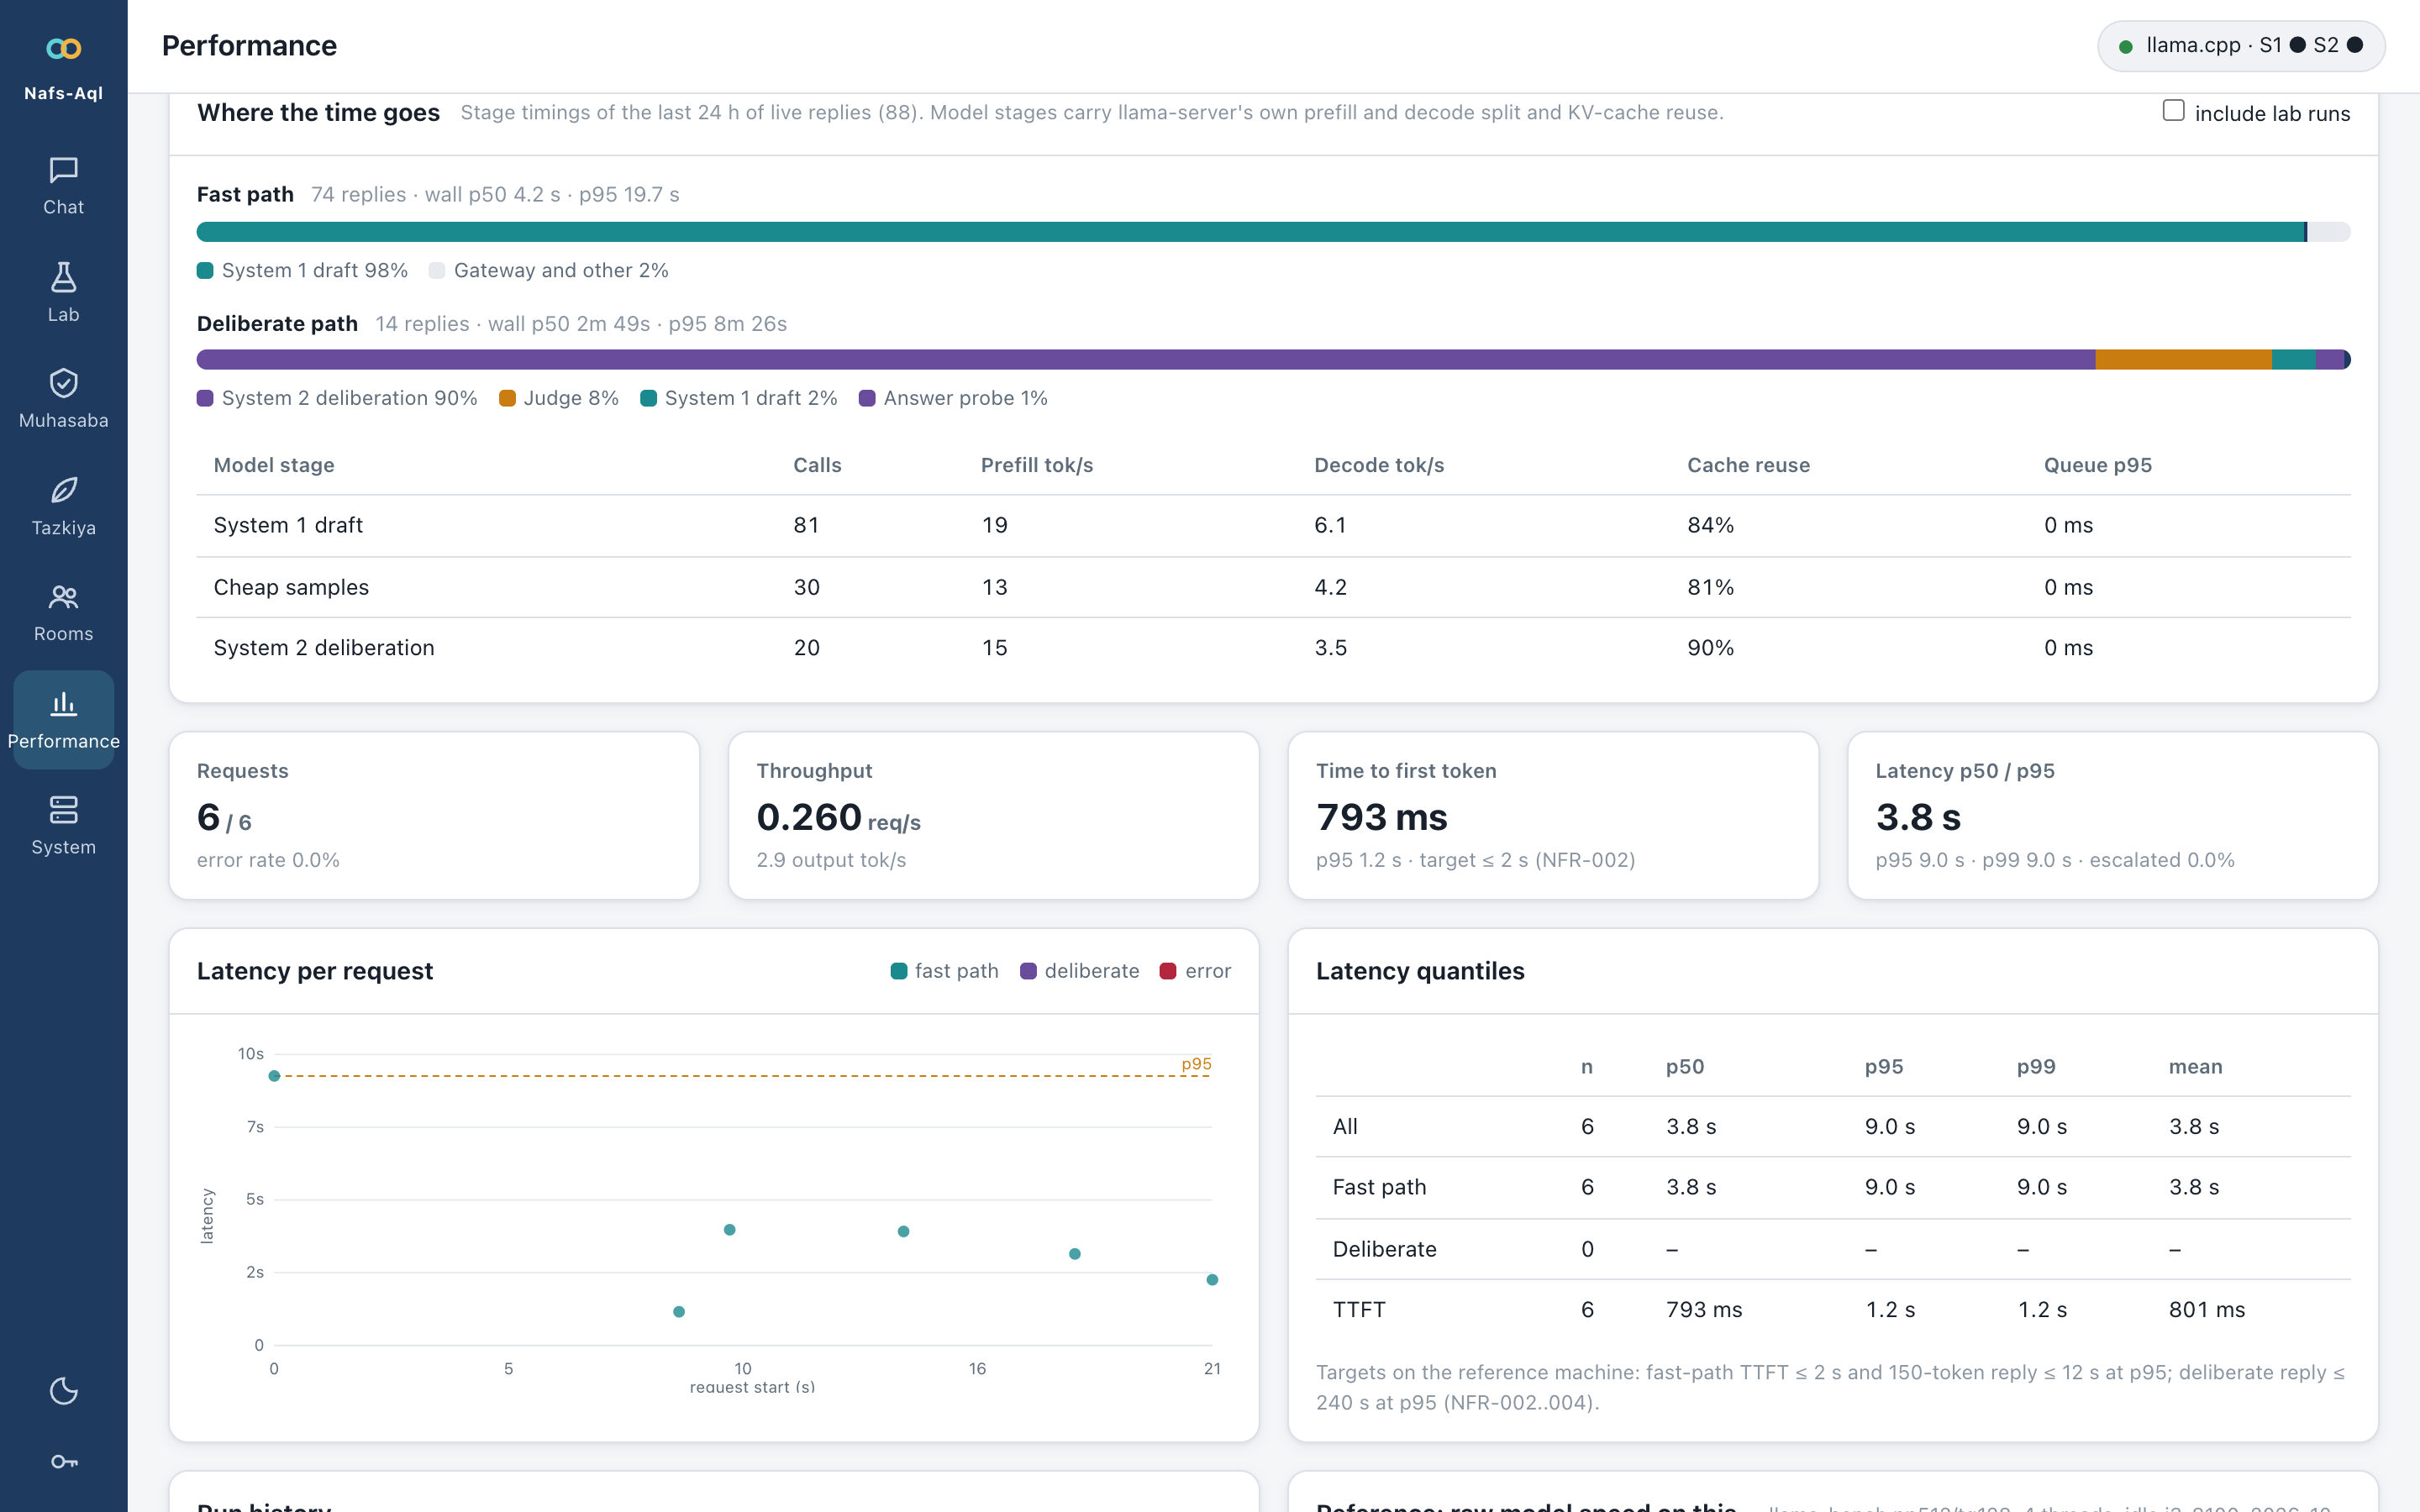
\includegraphics[width=0.48\textwidth]{../shared/screenshots/performance_stages.png}\hfill
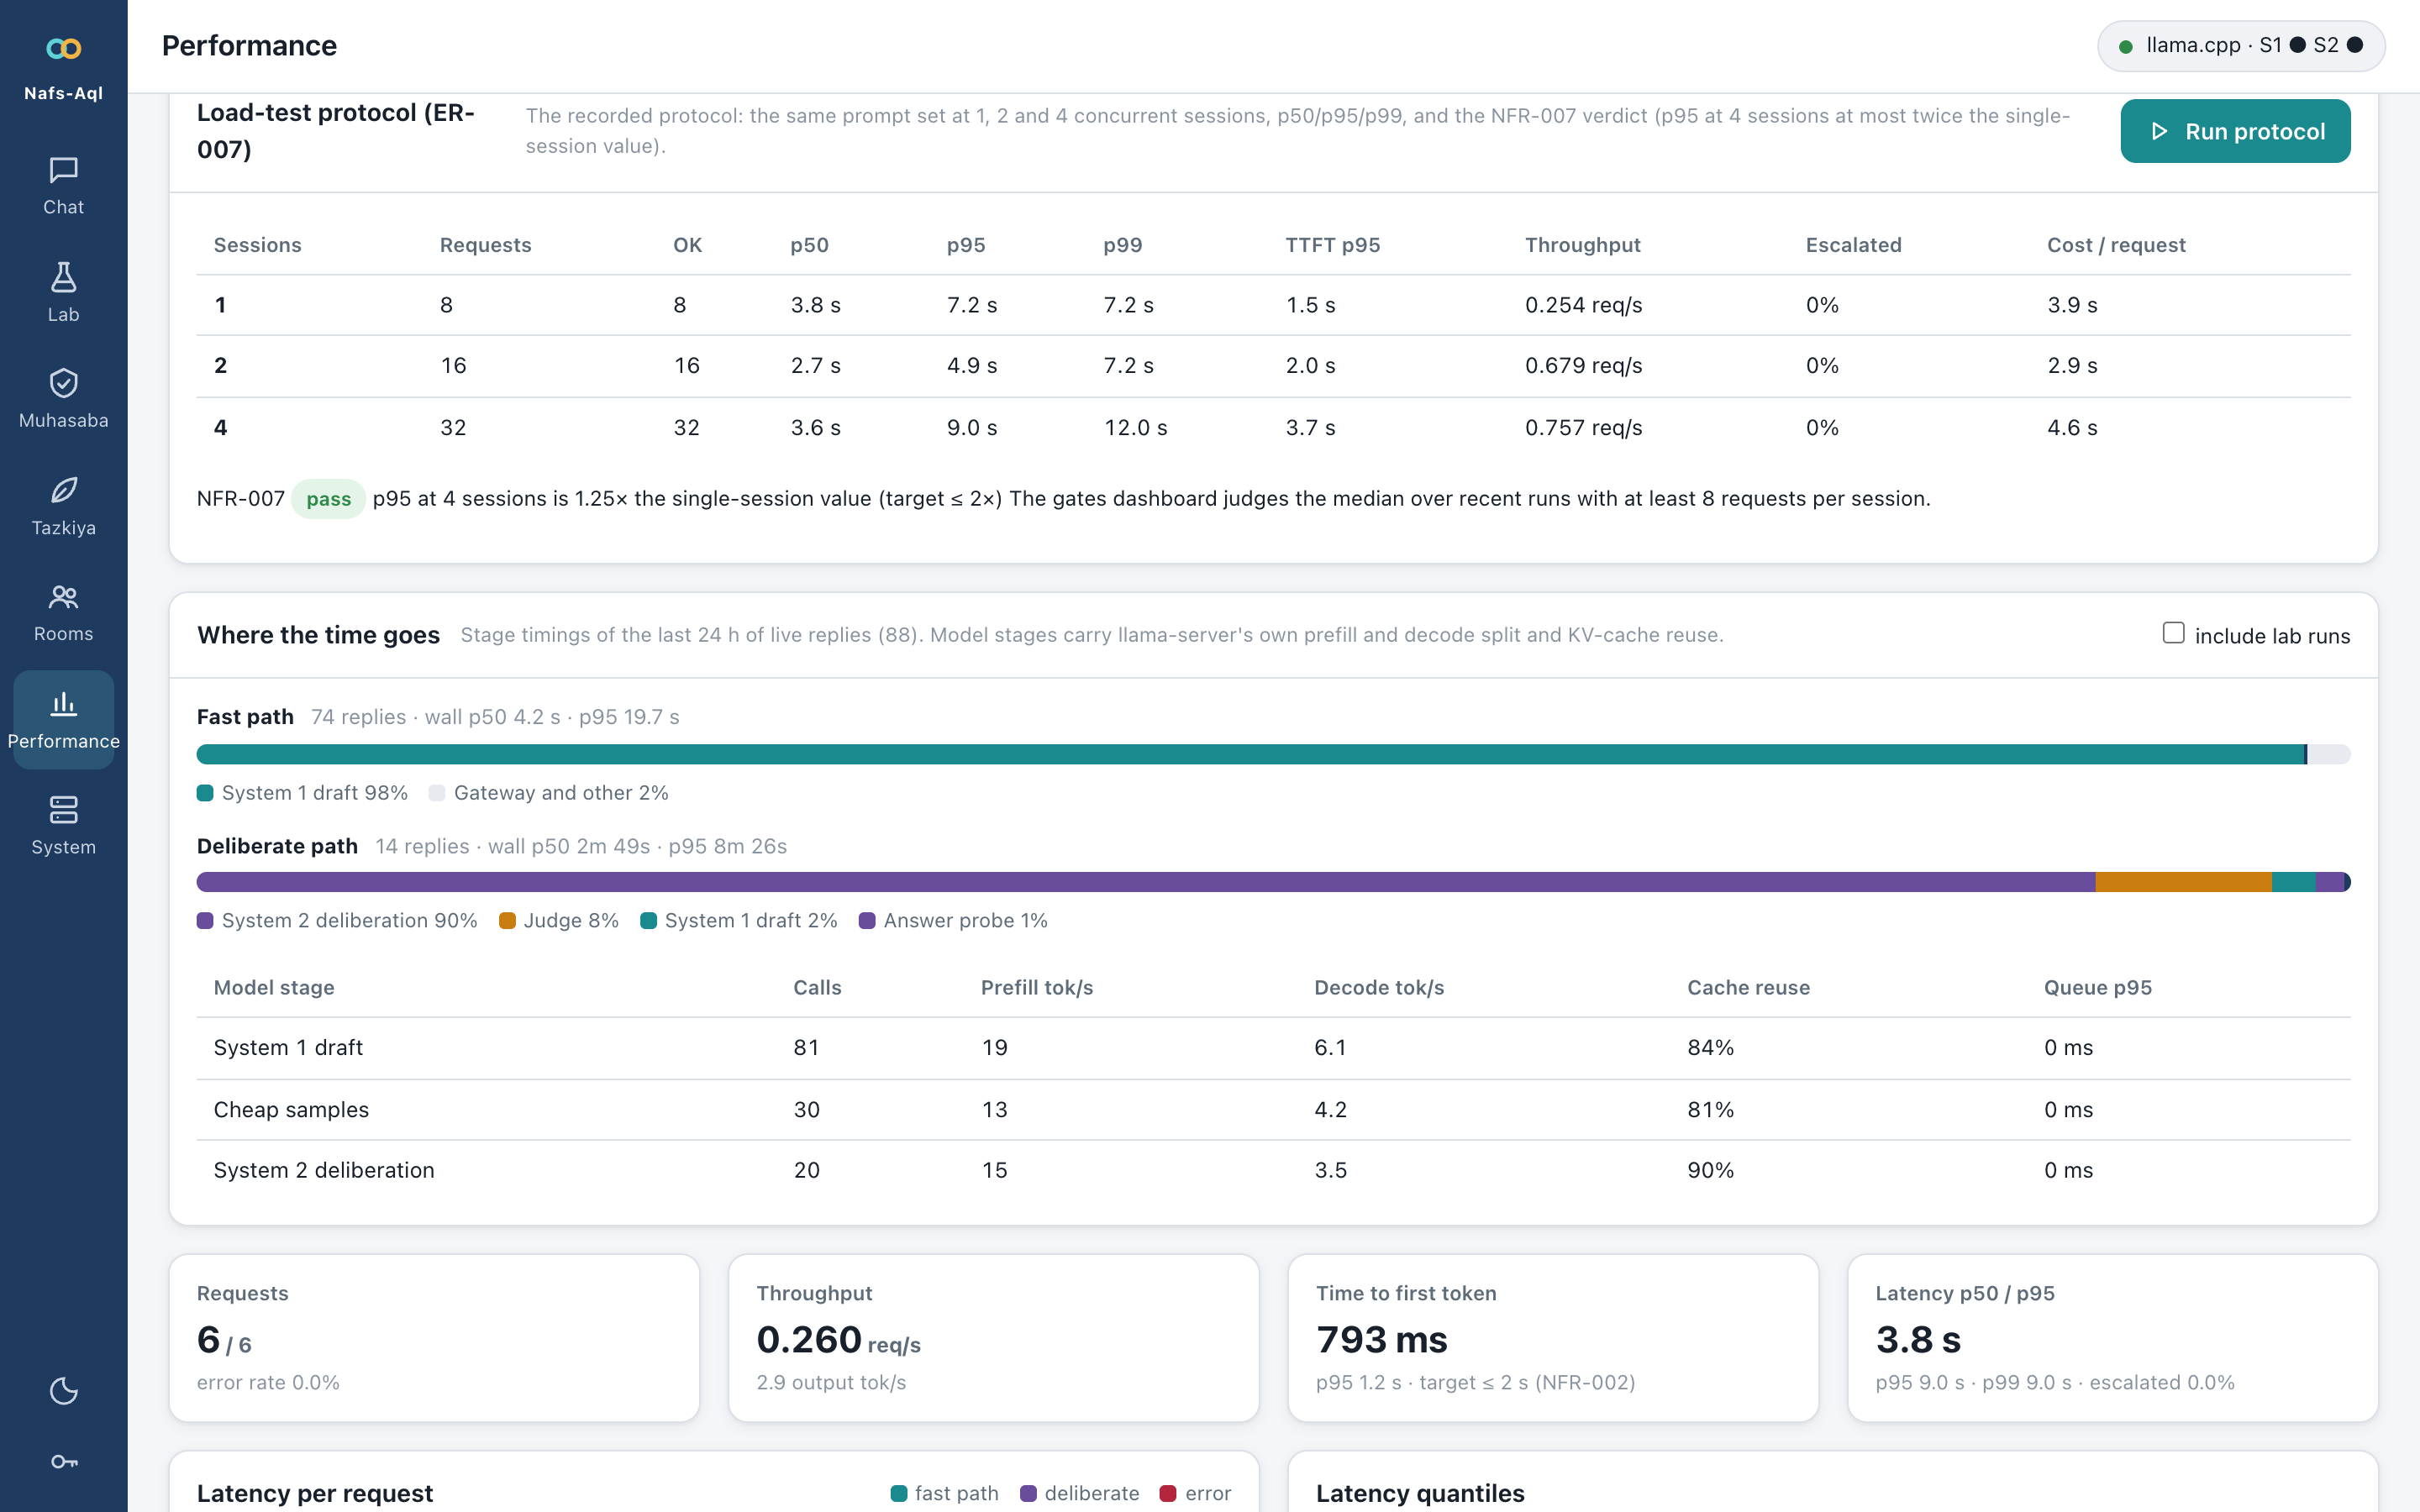
\includegraphics[width=0.48\textwidth]{../shared/screenshots/performance.png}
\caption{Performance page: where the time goes, from stage timings, with the engine's prefill and decode speed
and cache reuse (left); the load-test protocol at 1, 2 and 4 sessions with the NFR-007 verdict (right).}
\label{fig:ui-perf}
\end{figure*}

\textbf{Techniques and their measured effect.} Each change was accepted only after an interleaved A/B on the
reference machine (NFR-031):
\begin{itemize}
\item \emph{Skipping cheap samples when an exact verifier decides} (Theorem~1 makes them irrelevant): median
draft time fell from 13.4\,s to 7.9\,s.
\item \emph{Prompt-cache warm-up} at start-up, with llama-server's host-memory prompt cache: a cold first request
had 9.8\,s time to first token, a warm one about 1\,s.
\item \emph{Verifier warm-up}: the first verification after start-up fell from 0.45\,s to 3\,ms.
\item \emph{Early escalation} (FR-080): under the fixed rule, an open-ended draft whose running mean log-prob is
already below the threshold minus a margin is stopped and handed to System~2, instead of being generated to the
end, in the spirit of cost-aware cascades \cite{chen2023frugalgpt,yue2024cascades}. In the agreement study, \EarlyEscSummary{} (Table~\ref{tab:early}).
\item \emph{Sequential, uncertainty-gated samples}: the two agreement samples had run concurrently with
the draft, and three sequences on four cores tripled the factual fast path (12.6\,s median, 1.4\,s to first
token). They are now drawn after the draft and only when its mean log-prob lies within 0.10 of the threshold;
the path is 4.3\,s and 0.14\,s, the same as drawing no samples.
\item \emph{Four System~1 slots}: four sessions no longer queue behind three; batched decode makes the fourth
slot cheap.
\item \emph{No gain}, so not adopted:
  \begin{itemize}
  \item speculative decoding \cite{leviathan2023speculative} with a 0.6B draft model (6.5 against 7.3 tokens/s), because the draft model
  competes for the same cores and memory bandwidth;
  \item n-gram lookup;
  \item flash attention and a q8\_0 KV cache: a sequential run suggested a 30\% gain, which an interleaved repeat
  showed to be an ordering effect of the shared load.
  \end{itemize}
\end{itemize}

\begin{table}[t]
\centering\caption{Early-escalation agreement study (open-ended prompts)}\label{tab:early}
\EarlyEscTable
\end{table}

\textbf{Concurrency.} The load-test protocol (latest run \ProtocolRun, Table~\ref{tab:protocol}) gave a 4-session
p95 of \NfrSevenRatio{} times the single-session value. The gate judges NFR-007 on the median over recent eligible
runs (\NfrSevenPooled), because single runs on the shared host ranged from 1.25 to 2.48.

\begin{table}[t]
\centering\caption{Load-test protocol, fast path (run \ProtocolRun)}\label{tab:protocol}
\ProtocolTable
\end{table}

\textbf{Adaptive reasoning exit (FR-082).} The deliberate path is almost entirely System~2 reasoning, so the
second Phase~7 change shortens the reasoning itself, in the spirit of the 2026 early-exit methods
(DTSR, DEER, Dynasor-CoT) but with the design's own stopping signal. System~2 reasons in chunks on
llama-server's raw continuation endpoint, which keeps the prefix cached. At a reflection signal (``Wait'',
``Alternatively'', \ldots), with a minimum gap of 64 tokens and at the latest every 256 tokens, the reasoning
is closed provisionally and the model is asked for its answer in a few tokens. On a verifiable task the exact
verifier judges that probe and, if it passes, the reasoning stops; on factual tasks two consecutive agreeing
probes stop it. The final answer is then generated after the reasoning exactly as on the standard path, so the
exit changes only how much reasoning is generated, and the exit reason is recorded with the reply. A probe
costs 0.6--0.8\,s. In the paired Lab comparison (run \AdaptiveExitRun), \AdaptiveExitSummary.

\textbf{EAGLE-3 speculative heads} \cite{li2024eagle} for both models (AngelSlim, Apache-2.0) were converted and
measured in interleaved A/B runs (Table~\ref{tab:eagle}). On a GPU these heads give 1.7$\times$ because
verifying a draft is nearly free there. On four cores the verification pass costs real compute, and at the
measured acceptance of about half the drafted tokens neither system gained: System~1 1.04$\times$ greedy and
0.95$\times$ at the production temperature, System~2 0.99$\times$ on reasoning prompts; eight draft tokens were
slower than no speculation on both. The heads stay available
as an opt-in (\texttt{EAGLE=1}) for a host with more cores. Weight formats with AVX2 repack kernels
(Q4\_0, IQ4\_NL) remain to be measured the same way.

\begin{table}[t]
\centering\caption{EAGLE-3 speculative decoding, interleaved A/B on the reference CPU}\label{tab:eagle}
\resizebox{\columnwidth}{!}{\EagleTable}
\end{table}

\textbf{Weight formats.} Q4\_0 and IQ4\_NL use llama.cpp's AVX2 repack kernels, which read the weights in an
interleaved layout; Table~\ref{tab:quant} compares them with the production Q4\_K\_M on the same model
(interleaved \texttt{llama-bench} runs, 4 threads, host load recorded in the log).
\begin{table}[t]
\centering\caption{Weight formats, Qwen3-1.7B, llama-bench pp128/tg64}\label{tab:quant}
\QuantTable
\end{table}

\textbf{A smaller judge?} The rubric judge is the largest fixed cost on open questions once the adaptive exit
is in place (26--40\,s per answer on System~2). Scoring with System~1 instead would be about three times
faster, so it was measured with the rates harness on the same labelled items: \JudgeCompare. A judge that
accepts a quarter of the seeded wrong answers is not a soft verifier in the sense of Theorem~1, so the judge stays
on System~2; the backend remains a configuration option for hosts with a larger small model.

\textbf{vLLM backend.} The second serving profile, vLLM's CPU backend, now runs in Docker from the team's
\texttt{carstenz/vllm-smoke} image (vLLM 0.30, x86 CPU build) with Qwen3-1.7B serving both roles from the host's
Hugging Face weights, and the gateway switches between the two backend sets at run time. Two facts shaped the
recipe. First, the Docker VM exposes AVX2 only, where oneDNN has no BF16 kernels: in BF16 the engine loaded but
never returned a token, so the model runs in FP32 (6.8\,GB of weights). Second, the VM's memory cap matters: at
6\,GiB only 0.18\,GiB remained for the KV cache and at 10\,GiB with a 2\,048-token context the engine was OOM-killed
during its profiling pass, so the context, the prefill batch and the KV cache are kept small. The gateway-side
check, which drives every request path the orchestrator depends on against the backend, reports
\VllmCheckSummary. On four shared cores the three-vCPU VM is a correctness and portability profile, not a
speed contest with llama-server.

\subsection{Operations and the gates}
Monitoring and safety:
\begin{itemize}
\item \textbf{Drift and alerts} (Fig.~\ref{fig:ui-muh}): a two-sided CUSUM per domain on calibration error and
fast-path accuracy, with a shuffled negative control. Five alert rules run over live traffic only; evaluation
and load-test replies are tagged as lab traffic.
\item \textbf{Security:} \SecuritySummary. The suite found one high-severity issue, now fixed: sandboxed code
could signal other processes.
\item \textbf{Deployment checks:} \DeploySummary.
\end{itemize}
Table~\ref{tab:gates} lists the roadmap gates as evaluated from stored evidence. The gates that remain pending
need release-scale runs (thousands of paired items), GPU training, or the scholar review of the analogy text.

\begin{figure*}[t]
\centering
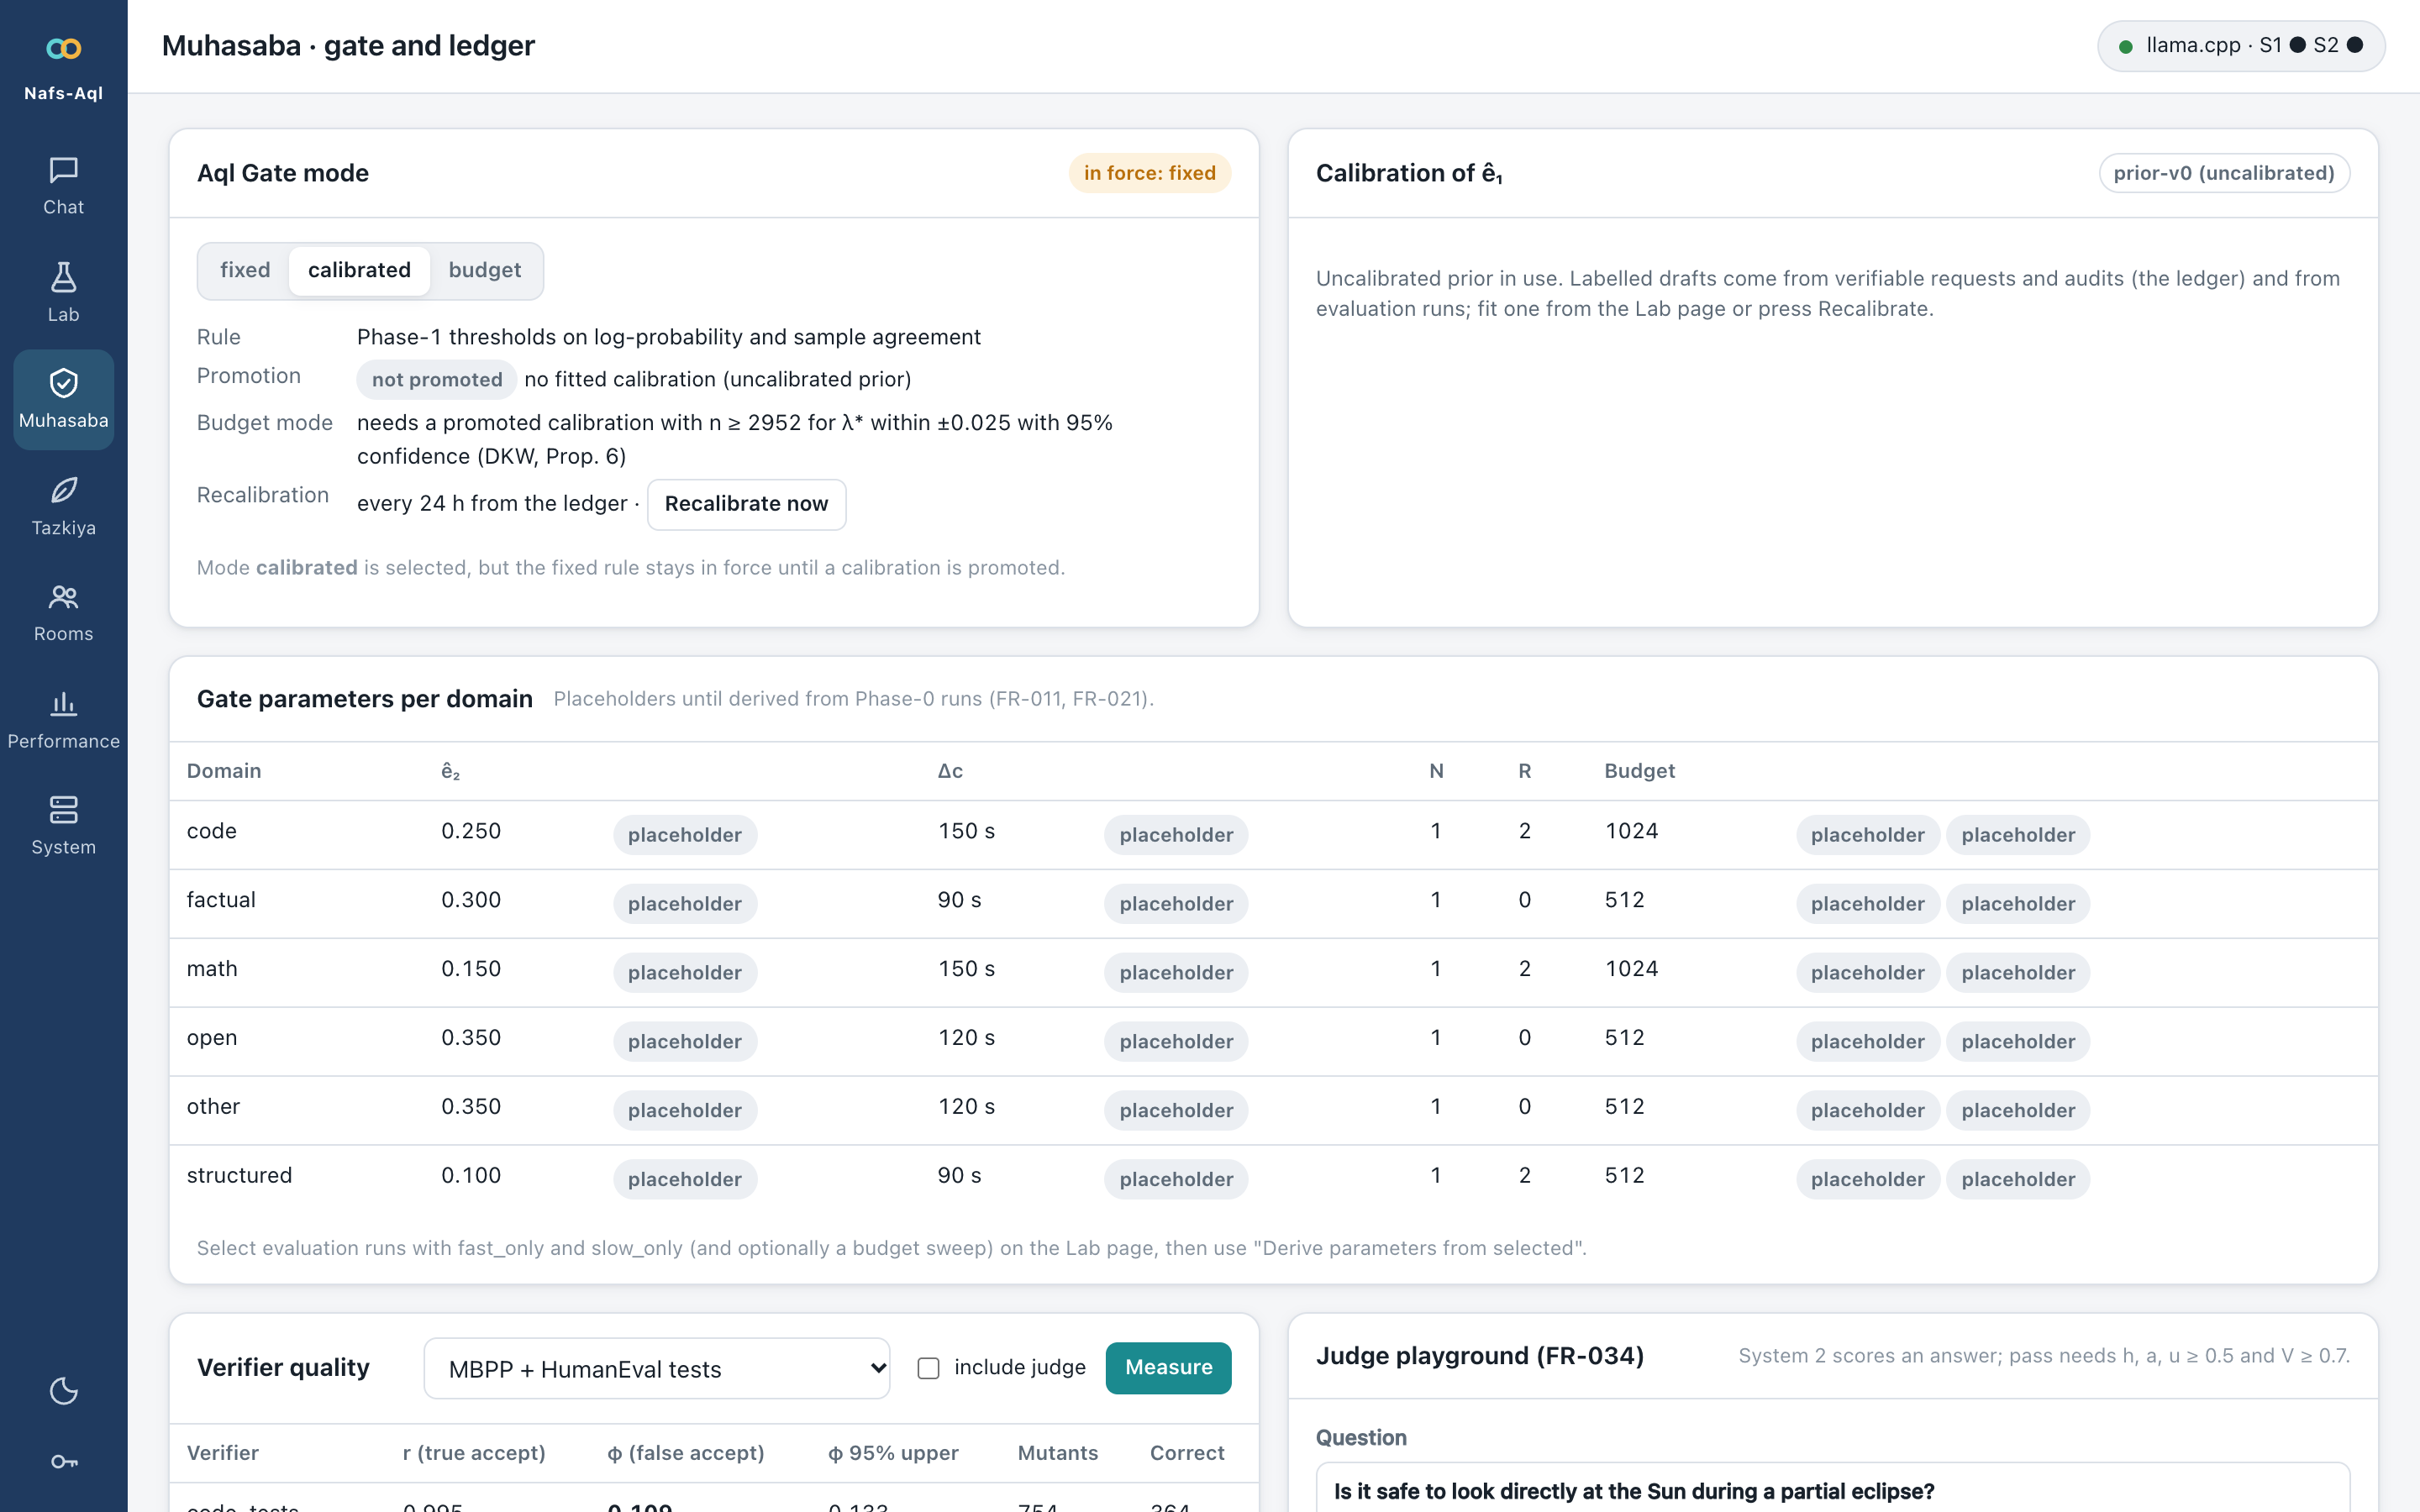
\includegraphics[width=0.48\textwidth]{../shared/screenshots/muhasaba.png}\hfill
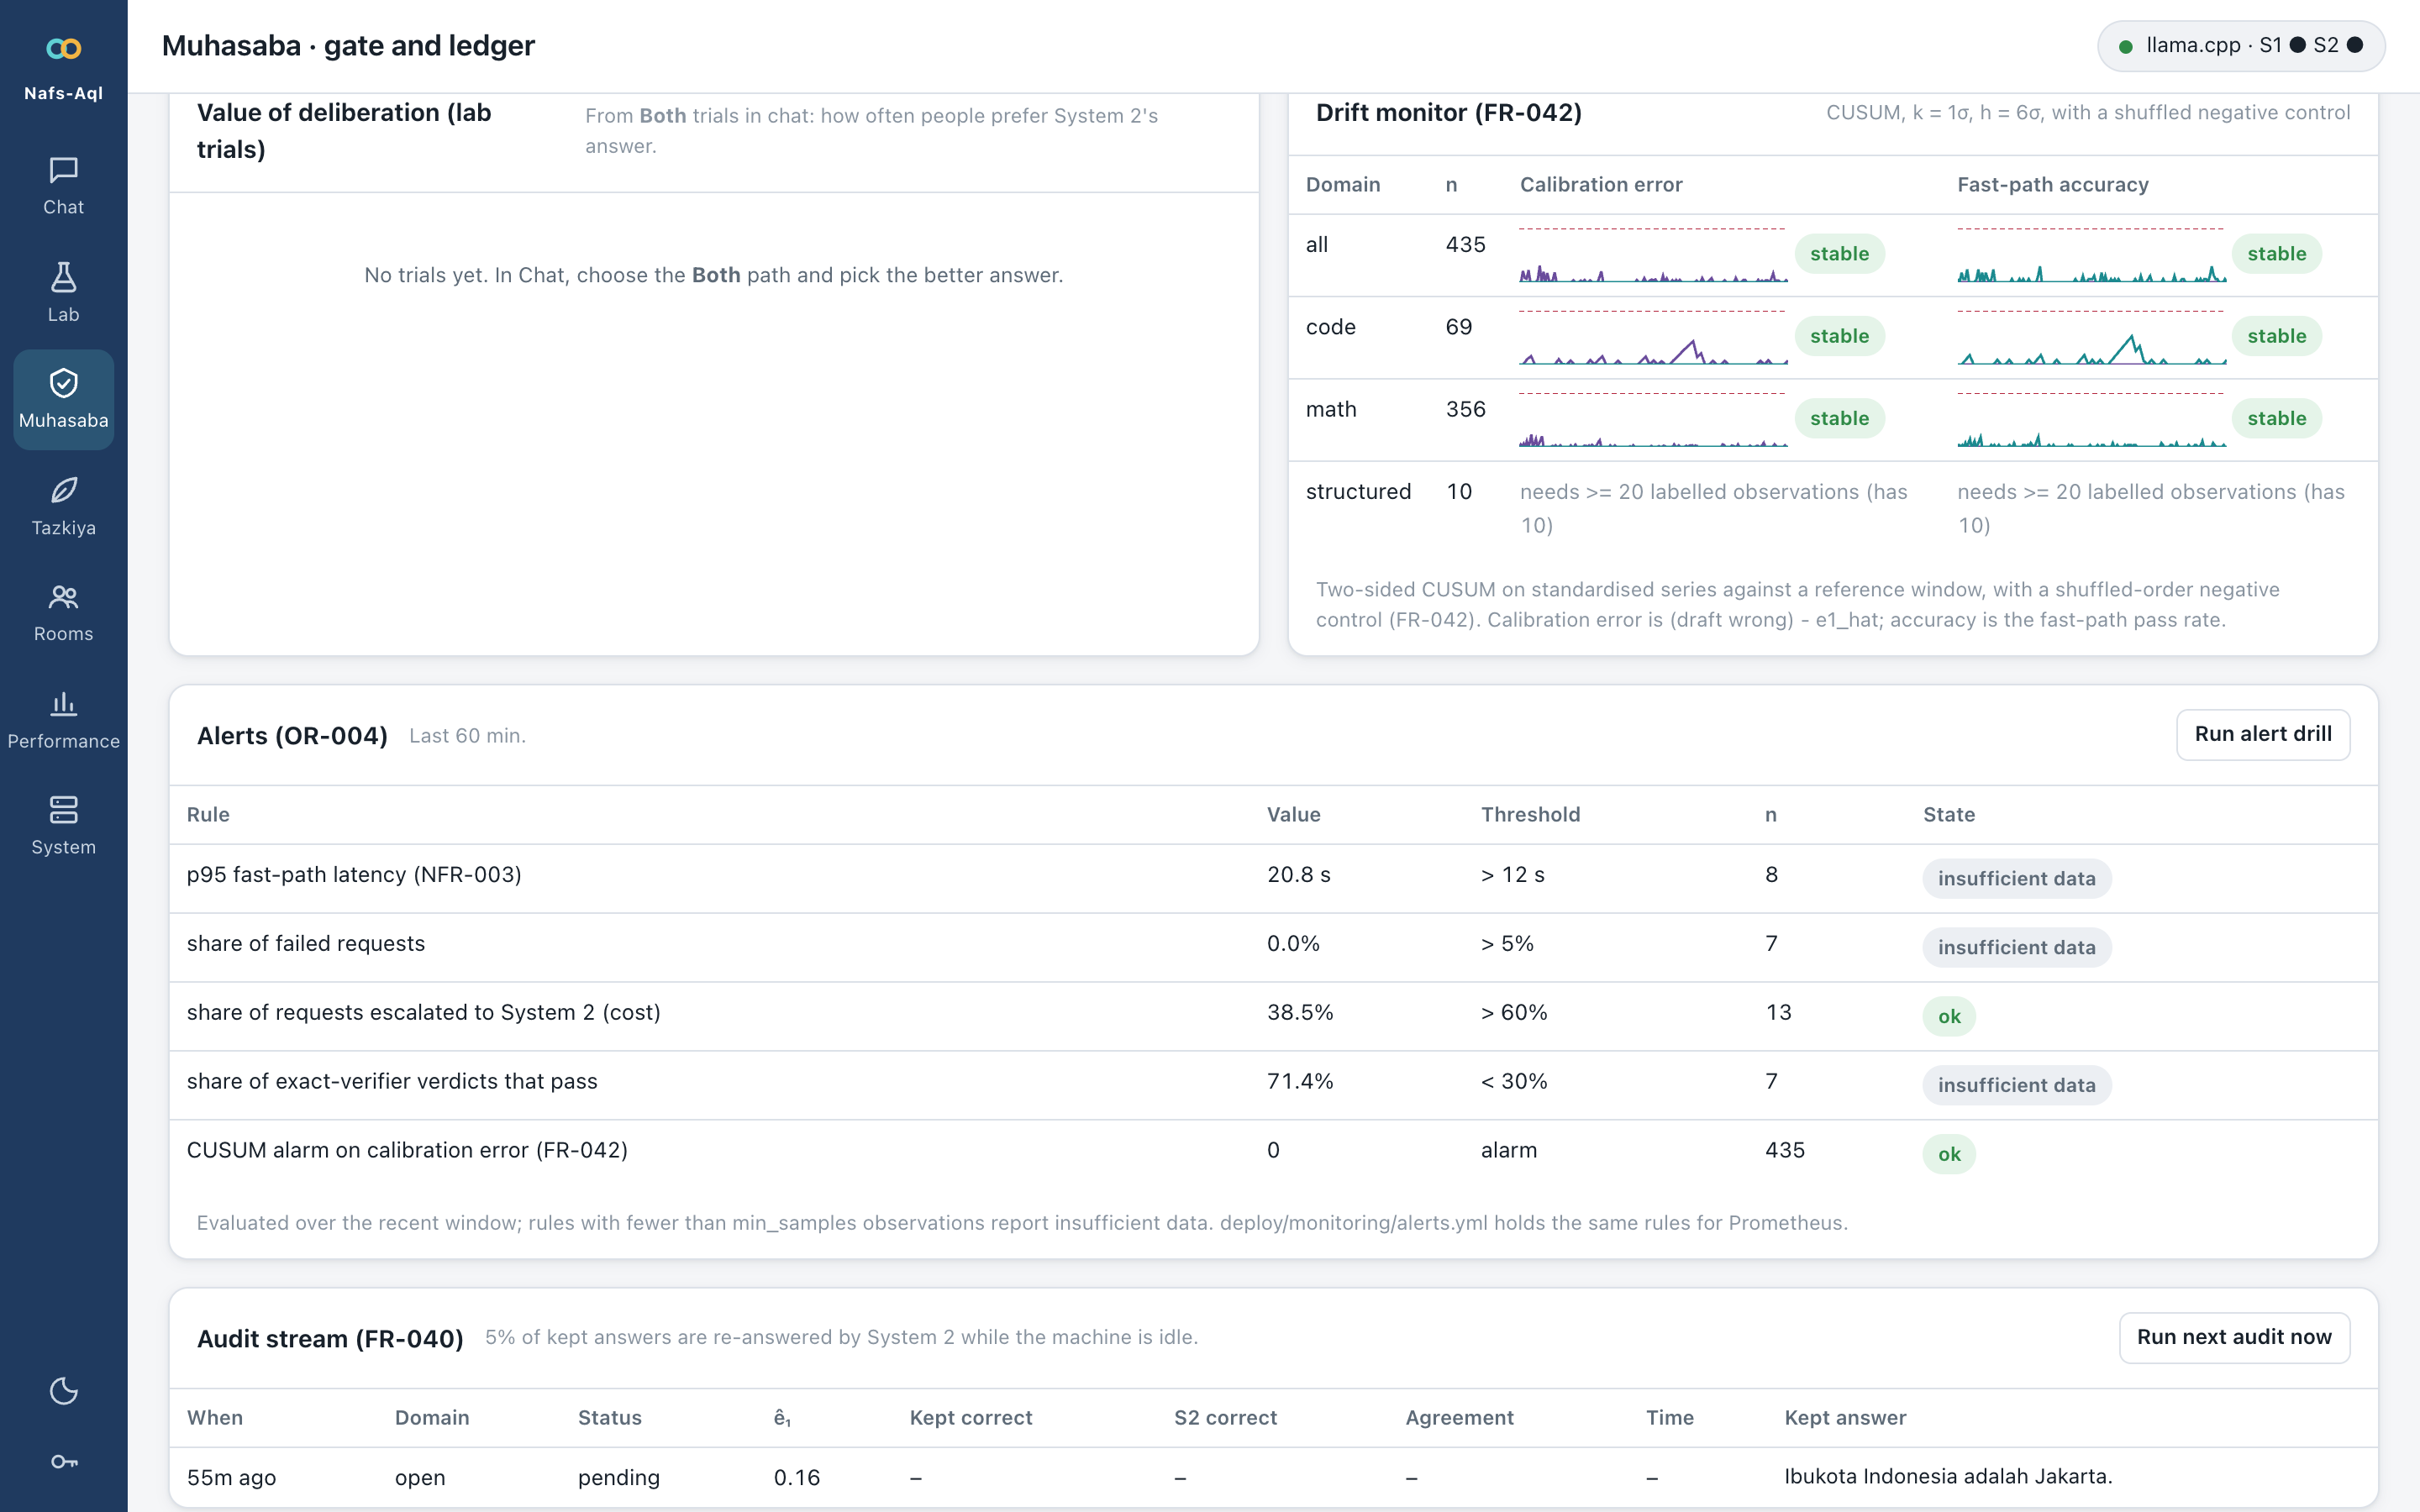
\includegraphics[width=0.48\textwidth]{../shared/screenshots/muhasaba_drift_alerts.png}
\caption{Muhasaba page: gate mode, promotion status and calibration (left); drift monitor and alert rules over
live traffic (right).}
\label{fig:ui-muh}
\end{figure*}

\begin{table*}[t]
\centering\caption{Roadmap gates evaluated from stored evidence (18 October 2026)}\label{tab:gates}
\small\GatesTable
\end{table*}
